\begin{exercise}
      {ID-666154ce84ca77a1eaaa7679c17c0644accdcc6d}
      {Diagonale}
  \ifproblem\problem
    Gib einen Term zur Berechnung der grauen Fläche in Abhängigkeit von $x$ und $y$ an.
    \begin{center}
      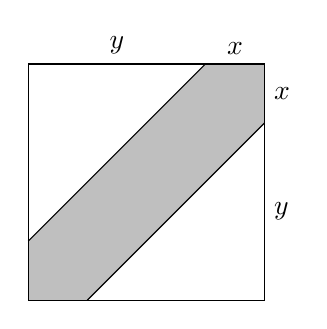
\begin{tikzpicture}[scale=0.75]
        % Doppelpfeil
        \fill[fill=black!25!white] (1, 0) -- (4, 3) -- (4, 4) -- (3, 4) -- (0, 1) -- (0, 0) -- cycle;
        \draw (1, 0) -- (4, 3);
        \draw (0, 1) -- (3, 4);
        % Quadrat
        \draw (0, 0) rectangle (4, 4);
        % Seitenlaengen
        \node[right] at (4.00, 1.50) {$y$};
        \node[above] at (1.50, 4.00) {$y$};
        \node[right] at (4.00, 3.50) {$x$};
        \node[above] at (3.50, 4.00) {$x$};
      \end{tikzpicture}
    \end{center}
  \fi
  %\ifoutline\outline
  %\fi
  %\ifoutcome\outcome
  %\fi
\end{exercise}
